\documentclass[8pt]{IEEEtran}

\usepackage{xcolor}
\definecolor{color1}{RGB}{146,212,245}
\definecolor{color2}{RGB}{78,184,237}
\definecolor{color3}{RGB}{2,154,229}
\definecolor{color4}{RGB}{1,108,160}
\definecolor{color5}{RGB}{0,54,92}
\definecolor{listbackground}{HTML}{D8F0FB}
\usepackage{listings}
\renewcommand{\lstlistingname}{Code-block}
\renewcommand{\lstlistlistingname}{List of \lstlistingname s}
\usepackage{textcomp}
\usepackage{tikz}
\usepackage{pgfplots}
\usepackage{inc/listings-golang}
\usepackage{inc/yaml}
\usepackage{inc/docker}
\lstset{
	backgroundcolor=\color{listbackground},
	tabsize=4,
	language=Golang,
    language=yaml,
    language=docker,
    language=docker-compose,
	rulecolor=,
	language=matlab,
        basicstyle=\scriptsize,
        upquote=true,
        captionpos=b,
        aboveskip={1.5\baselineskip},
        columns=fixed,
        showstringspaces=false,
        extendedchars=true,
        breaklines=true,
        prebreak = \raisebox{0ex}[0ex][0ex]{\ensuremath{\hookleftarrow}},
        frame=single,
        showtabs=false,
        showspaces=false,
        showstringspaces=false,
        identifierstyle=\ttfamily,
        keywordstyle=\color[rgb]{0,0,1},
        commentstyle=\color[rgb]{0.133,0.545,0.133},
        stringstyle=\color[rgb]{0.627,0.126,0.941},
}

\usepackage{graphicx}
\usepackage{amsmath}
\usepackage{url}
\usepackage[utf8]{inputenc}
\usepackage{glossaries}
\usepackage{float}
\usepackage[english]{babel}
\usepackage[hidelinks]{hyperref}
\usepackage[capitalise,noabbrev]{cleveref}
\crefname{listing}{Code-block}{Code-block}
\Crefname{listing}{Code-block}{Code-block}
\providecommand{\tightlist}{%
  \setlength{\itemsep}{0pt}\setlength{\parskip}{0pt}}
\usepackage[backend=bibtex,
  bibencoding=utf8,style=ieee]{biblatex}
\addbibresource{bib/bib}



\begin{document}

\pagenumbering{roman}
\title{Assignment GA3. Musical Key identification}
% author names and affiliations
% use a multiple column layout for up to three different
% affiliations
\author{\IEEEauthorblockN{Miguel Pinheiro}
\IEEEauthorblockA{201705172} 
\and
\IEEEauthorblockN{Diogo Remião}
\IEEEauthorblockA{201706373}}

% make the title area
\maketitle



\section*{Caracterização geral da simulação}

%sistemas
\noindent
Este \textit{Call center} tem dois sistemas separados:
\begin{itemize}
    \item Sistema GP, que atende todas as chamadas e reencaminhada chamadas para o sistema AS se necessário
    \item Sistema AS, que atende as chamadas de carácter específico reencaminhadas pelo sistema GP
\end{itemize}

%parametros
\noindent
Definimos os seguintes parâmetros de funcionamento do \textit{Call center}:
\begin{itemize}
    \item Nº de servidores no sistema GP
    \item Nº de servidores no sistema AS
    \item Tamanho da fila de espera no sistema GP (infinita no sistema AS)
\end{itemize}


%chamadas
\noindent
Sendo esta uma simulação de um \textit{Call center}, duas situações podem acontecer:
\begin{itemize}
    \item 30\% de probabilidade de uma chamada apenas precisar de ser atendida no sistema GP.
    \item 70\% de probabilidade de uma chamada precisar de ser no sistema GP e depois no sistema AS.
\end{itemize}


%eventos
\noindent
Distinguem-se 3 tipos de eventos no sistema:
\begin{itemize}
    \item CHEGADA: Uma chamada que chega a um sistema, sem discriminação do seu tipo.
    \item PARTIDA\_GP: Uma chamada que é atendida no sistema GP e depois sai do sistema.
    \item PARTIDA\_AS: Uma chamada que é atendida no sistema GP e entra no sistema AS / Chamada que é atendida no AS
\end{itemize}

As distinção entre PARTIDA\_GP e PARTIDA\_AS é apenas relevante no sistema GP. No sistema AS, faz-se uma abstração para apenas PARTIDA.

Cada evento tempo um \textit{timestamp} associado.
No evento de \textbf{CHEGADA}, define o momento em que chegou.
Nos de \textbf{PARTIDA}, o momento em que partiu.
Este valores são gerados conforme indicado no guião.
\newline

%listas
\noindent
A \textbf{lista\_eventos\_gp} é uma fila onde serão guardados todos os eventos que chegam ao sistema GP.
A \textbf{lista\_espera\_gp} é uma fila onde serão guardados todos os eventos que estão num determinando momento na fila de espera para serem processados pelo sistema GP.
Um evento é colocado na fila de espera quando todos servidores estão ocupados.
Se a fila estiver cheia, a chamada é considerada como perdida e removida.

A \textbf{lista\_eventos\_as} e a \textbf{lista\_espera\_as} têm a mesma funcionalidade mas para o sistema AS.
Um evento é colocado na fila de espera quando o os servidores estão ocupados.
A fila de espera é infinita, pelo que não haverá chamadas perdidas.

\section*{Descrição do funcionamento do algoritmo}

\begin{figure}[H]
    \centering
    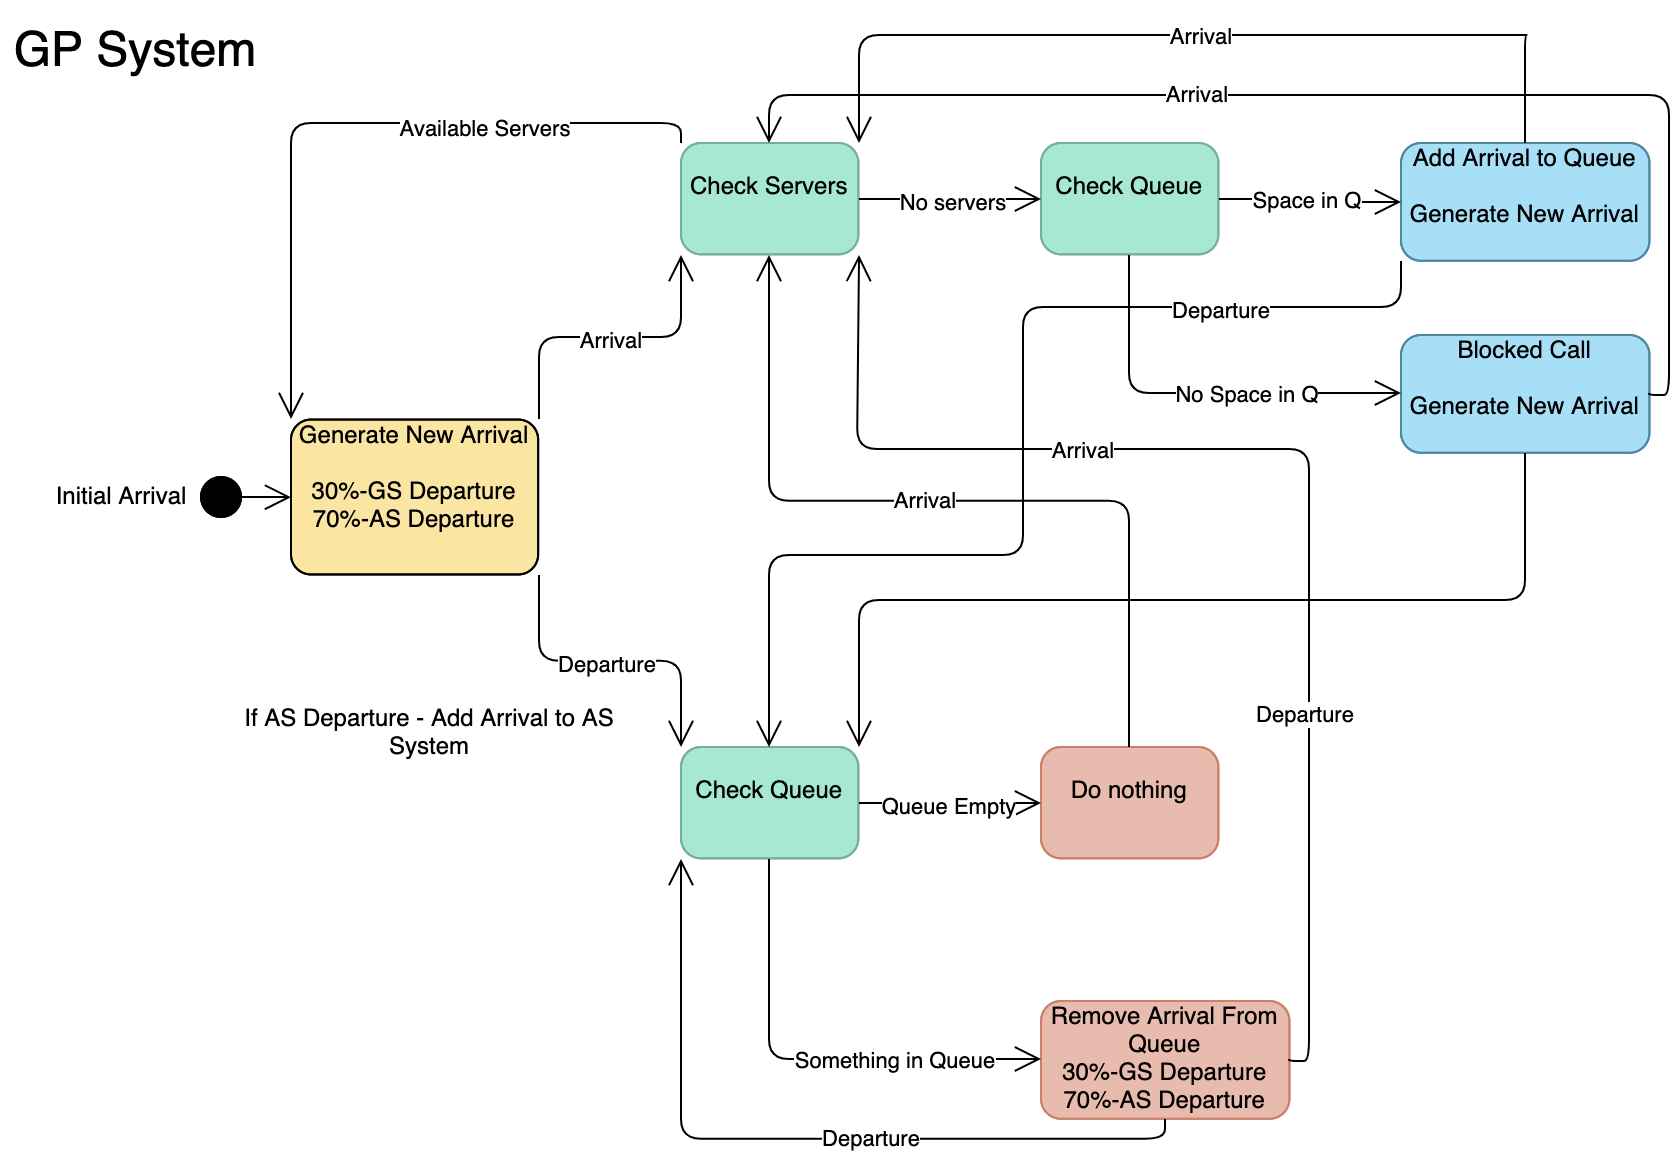
\includegraphics[width=.9\linewidth]{figs/intro/sm_gp.png}
    \caption{Máquina de estados do Sistema General Purpose}
    \label{fig:sm_gp}
\end{figure}

A figura \ref{fig:sm_gp} é uma máquina de estados que representa o algoritmo do \textbf{sistema GP}.
Primeiro verifica-se o tipo de evento que está na \textbf{lista\_eventos\_gp}.

Se o evento for de \textbf{CHEGADA}, verifica-se o estado do sistema.
Se os servidores estivem ocupados, verifica-se a fila de espera.
Se esta estiver livre, esse evento é colocado na \textbf{lista\_espera\_gp}.
Caso contrário é bloqueado.
Novas \textbf{CHEGADAS} são sempre geradas quando se processa uma \textbf{CHEGADA}.

Se o evento for de \textbf{PARTIDA}, verifica-se se há algum evento na \textbf{lista\_espera\_gp}.
Se houver, começa-se imediatamente a processar esse evento, gerando uma nova \textbf{PARTIDA}.
Caso contrário, passa-se para o próximo evento na \textbf{lista\_eventos\_gp}.

Por fim, considera-se que uma \textbf{CHEGADA} é gerada no \textbf{sistema AS} quando é processada uma \textbf{PARTIDA\_AS}.


\noindent
\newline
O princípio de funcionamento do sistema AS é semelhante, ilustrado na figura \ref{fig:sm_as}. Destaca-se alguma diferenças.


As \textbf{CHEGADAS} não são geradas no \textbf{sistema AS}, mas sim no \textbf{sistema GP}, pelo que o sistema pode ficar inativo, algo que não acontece com o \textbf{sistema GP}.
Além disso, não existe a risco de uma chamada ser bloqueada pois a fila é infinita.
A \textbf{lista\_eventos\_as} é constantemente verificada para detetar se alguma chamada foi reencaminhada para ser atendida pela sistema. Quando o sistema fica \textit{idle}, volta a este estado.

As \textbf{PARTIDAS} são geradas também quando uma CHEGADA é processada, no entanto a distribuição temporal é diferente das duas partidas do sistema GP.

\begin{figure}[H]
    \centering
    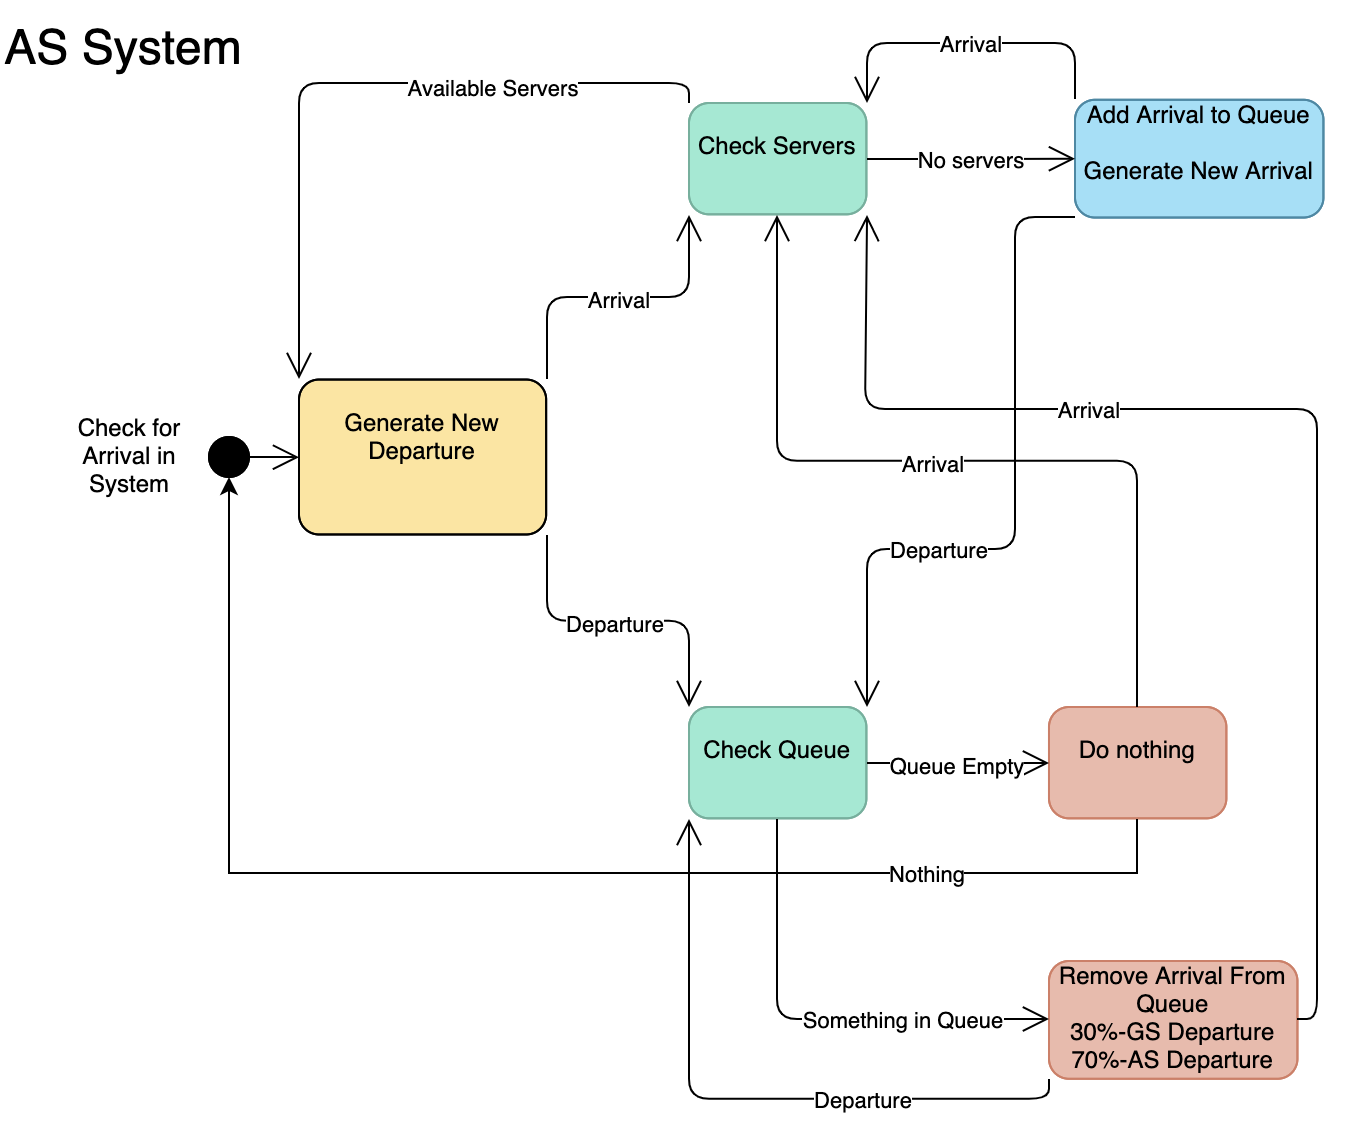
\includegraphics[width=.7\linewidth]{figs/intro/sm_as.png}
    \caption{Máquina de estados do Sistema Area Specific}
    \label{fig:sm_as}
\end{figure}

\section*{Estimativa do tempo de espera}

De forma a puder fornecer uma previsão do tempo de espera a cada chamada que chega, é necessário adotar um algoritmo de \textit{running average}.
Este algoritmo permite o calculo dinâmico da média do tempo de espera a cada chamada que chega, atualizando a cada iteração.

A estimativa do tempo de espera começa a 1. Quando uma chamada chega, duas situações podem acontecer:
\begin{itemize}
    \item Chamada é imediatamente atendida, pelo que o delay é 0 segundos.
    \item Chamada é colocada na fila de espera. O delay é calculado no momento em que a chamada sai da fila de espera.
\end{itemize}

Quando um novo valor de delay é obtido, uma nova média é calculada.
Por exemplo, com um delay de 60 segundos, a nova média será $\frac{0+60}{2}=30s$.
Quando uma nova chamada chegar, a estimativa de tempo de espera apresentada será de 30 segundos.
A cada iteração, este valor é atualizado.
Como este sistema tende para a estabilidade, este valor aproxima-se para um valor constante, que vai fornecer uma previsão mais sólida quantas mais chamadas forem atendidas.


\section*{Resultados da simulação}

De modo a garantir os objetivos de performance mínimos, necessitamos de pelo menos \textbf{4 Servidores GP}, \textbf{2 Servidores AS} e \textbf{Fila de Espera GP de tamanho 2}.
Os seguintes parâmetros foram obtidos:
\begin{center}
    \begin{tabular}{||c|c c||} 
    \hline
    Parâmetro & Mínimo & \textbf{Obtido} \\
    \hline\hline
    Delay Prob & 30\% & \textbf{12.83\%}\\ 
    \hline
    Blocked Prob & 2\% & \textbf{1.35\%}\\
    \hline
    Avrg Delay GS& 30s & \textbf{23.4s}\\
    \hline
    Avrg Delay Total & 60s & \textbf{24s} \\
    \hline
   \end{tabular}
\end{center}

O \textit{Bottleneck} deste sistema é o \textbf{Avrg Delay GS}, que está muito mais próximo do limite do que os restantes parâmetros.
Um relaxamento deste parâmetro para 40 segundo permitia que fosse utilizado apenas 3 servidores GP.

Com estes parâmetros, foram gerados histogramas que representam a distribuição dos atrasos e dos erros de previsão.

\begin{figure}[H]
    \centering
    \begin{subfigure}[b]{0.49\textwidth}
        \centering
    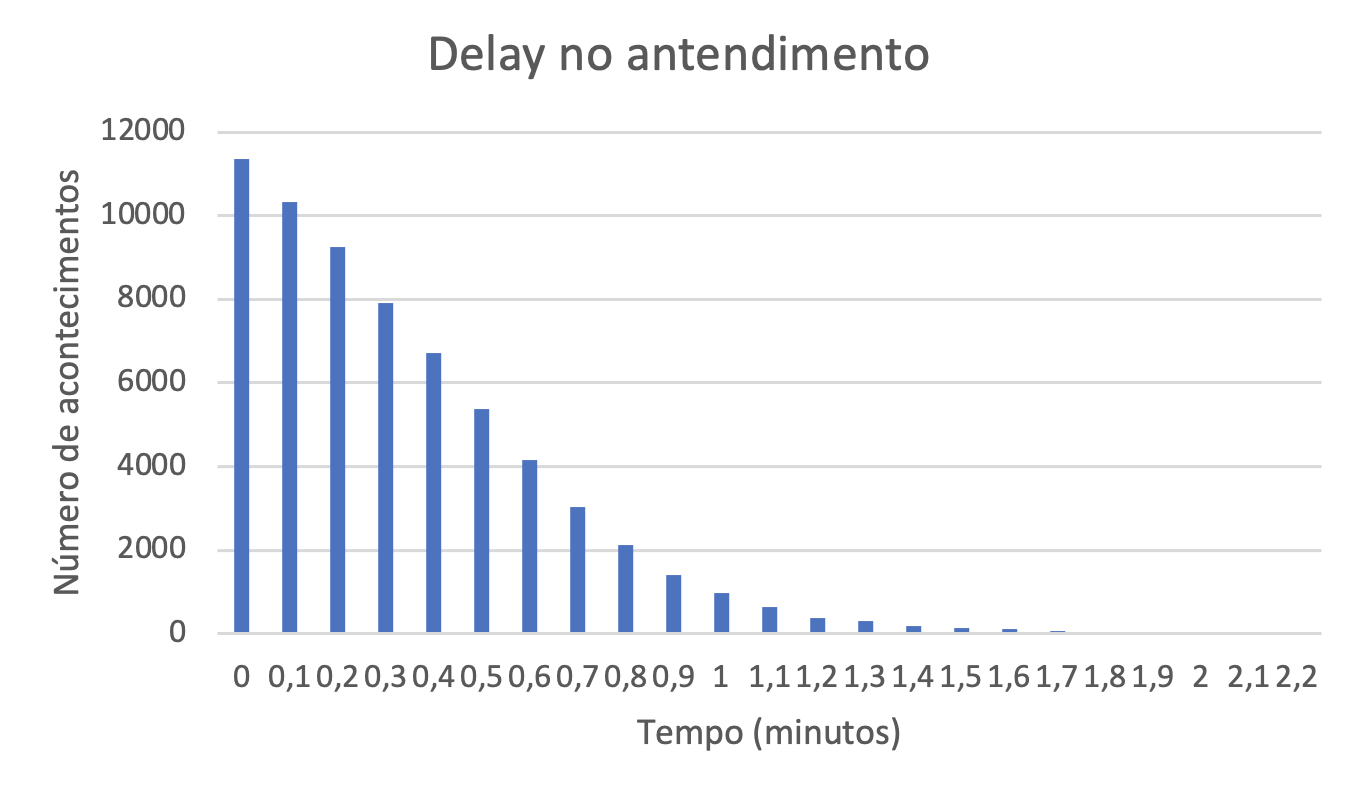
\includegraphics[width=\linewidth]{figs/intro/histo_delay.png}
    \caption{Distribuição dos delays no sistema}
    \label{fig:histo_delay}
    \end{subfigure}
    \hfill
    \begin{subfigure}[b]{0.5\textwidth}
        \centering
    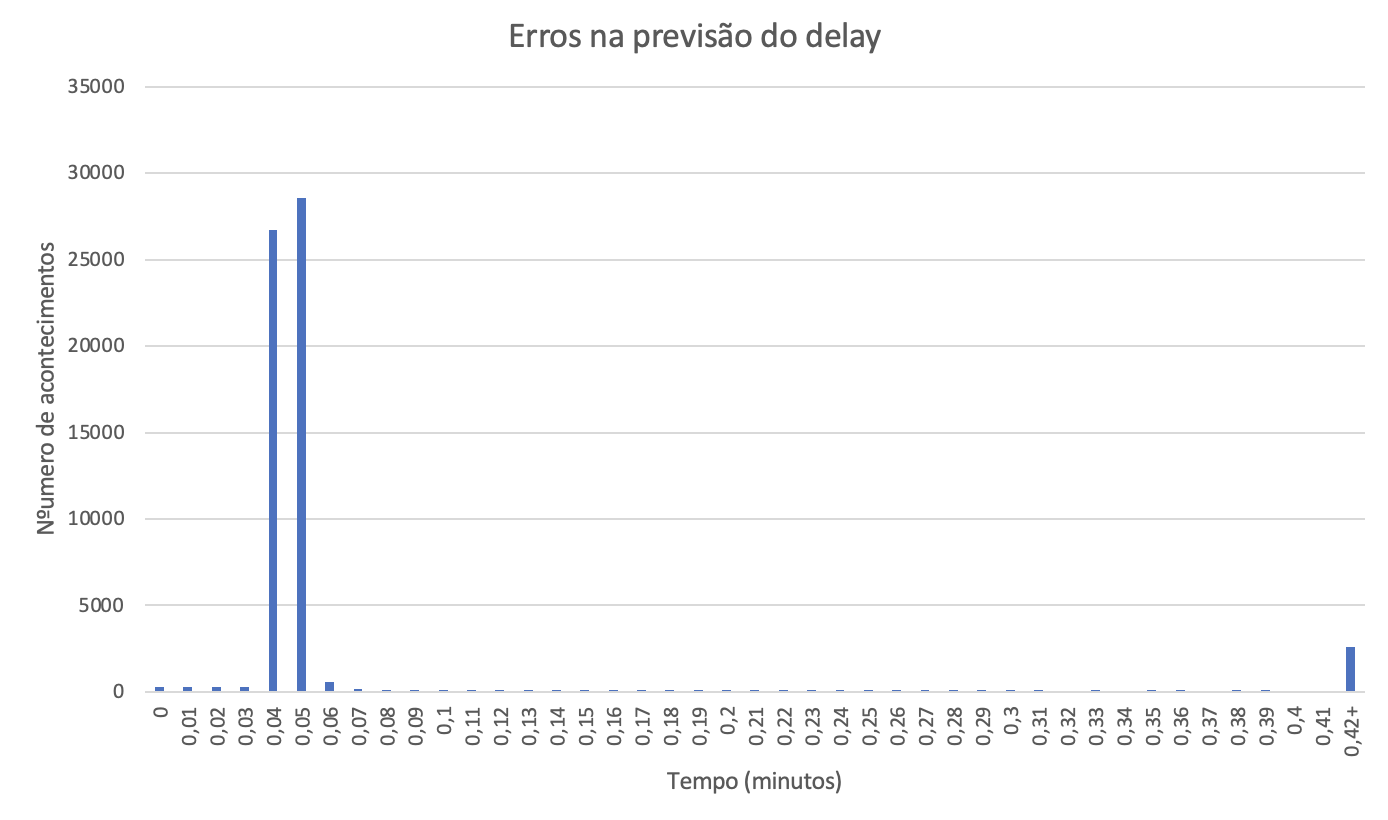
\includegraphics[width=\linewidth]{figs/intro/histo_erro.png}
    \caption{Distribuição do erro de previsão no sistema}
    \label{fig:histo_erro}
    \end{subfigure}
       \label{fig:histogramas}
\end{figure}

A distribuição dos dos \textit{Delays} aproxima-se de uma distribuição exponencial, pois este sistema é estável, ou seja, $\rho<1$.
Se $\rho>1$, esta distribuição seria crescente pois o tempo de espera iria aumentar com o tempo. Os delays 0 não estão representados.

Uma analíse do histograma dos erros indica que grande parte dos erros foi na ordem dos 0.04-0.06 segundos, que é sensivelmente o valor médio de atraso.
Mais uma vez, o facto do sistema ser estável fez com que os erros obtidos fossem da ordem da média.

\section*{Análise de Sensibilidade e Estimador}

\begin{figure}[H]
    \begin{floatrow}
    \ffigbox{%
    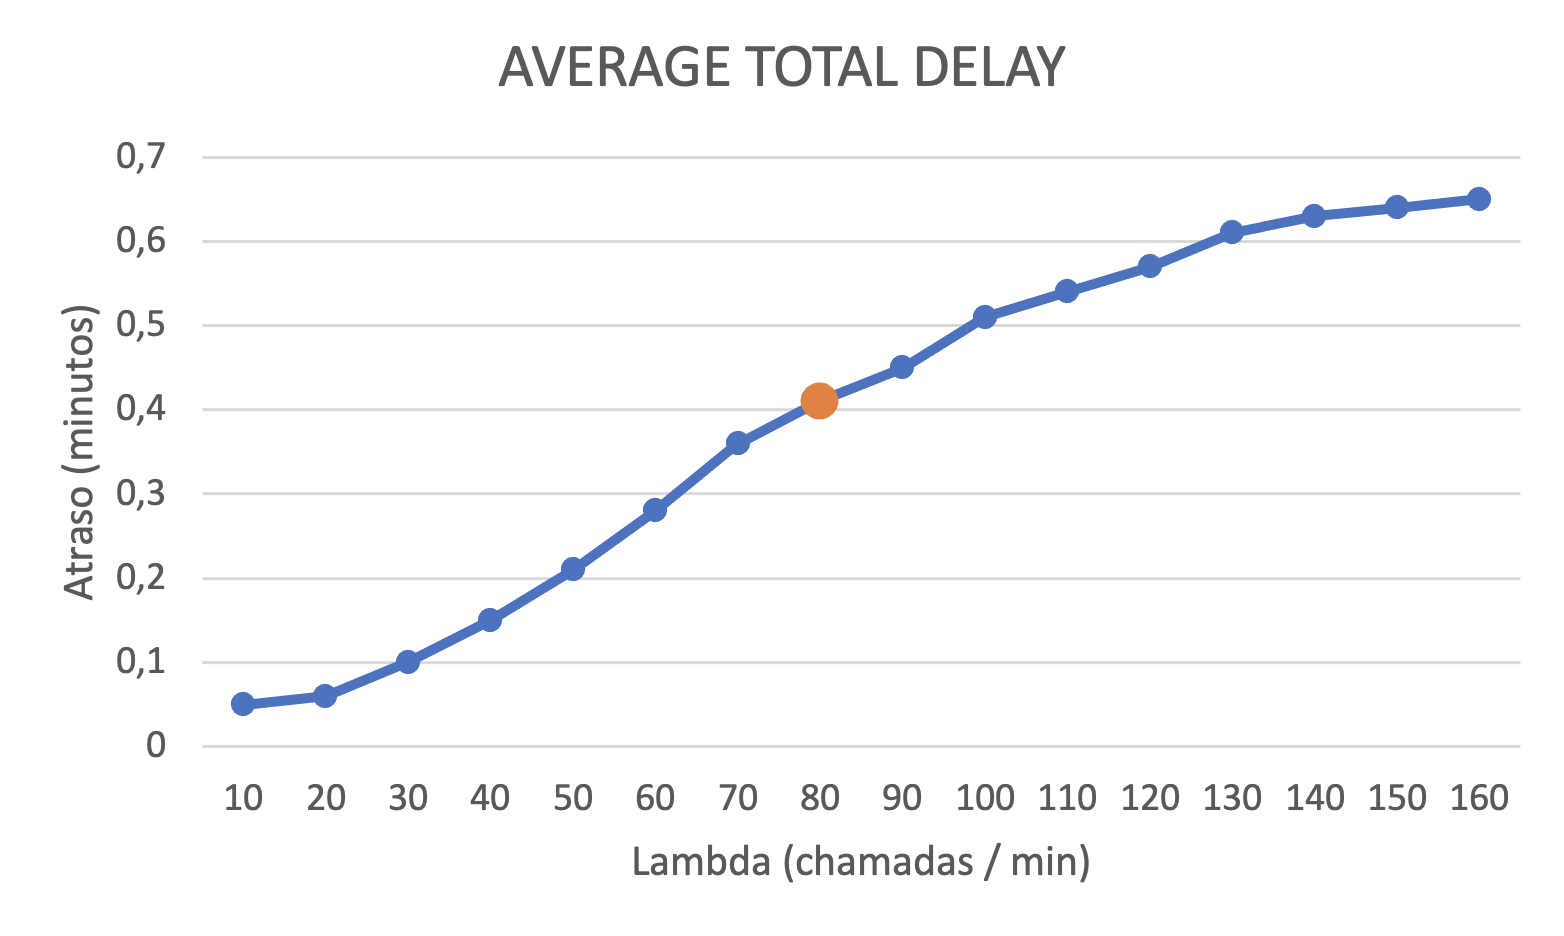
\includegraphics[width=.9\linewidth]{figs/intro/total_delay.png}
    }{%
    \caption{Total Delay time com variação da frequência de chegadas}
    }
    \capbtabbox{%
    \begin{tabular}{||c|c||} 
        \hline
        Intervalo de Confiança & 90\% \\
        \hline
        Número de Amostras & 30 \\
        \hline
        Graus de Liberdade & 29 \\
        \hline
        t (Student) & 1.6973 \\
        \hline
        Média & 0.410105 \\
        \hline
        Desvio Padrão & 0.005534535\\
        \hline
        Limite Inferior & 0.408389941 \\
        \hline
        Limite Superior & 0.411820059 \\
        \hline
       \end{tabular}
    }{%
    \caption{Estimador do Average Total Wait Time com intervalo de confiança de 90\% - 2 Tail}
    }
    \end{floatrow}
\end{figure}


A figura 4 mostra a relação entre a \textit{Arrival Rate} e o Atraso do sistema.
Observamos, como esperado, que o atraso tende para 0 à medida que se diminúi a \textit{Arrival Rate}.

À medida que o valor aumenta, o atraso tendo para um valor próximo de 0.65 minutos.
Isto deve-se ao facto da fila de espera ter tamanho limite.
O tempo que uma chamada tem que esperar se estiver no fim da fila não aumenta pois tem sempre o mesmo número de chamadas à sua frente.
O que aumenta é a probabilidade de perder a chamada. É deste modo de esperar este comportamento.

Também foi calculado um estimar para o Average Total Wait Time com base em 30 amostras do parâmetro.


\section{Related Work} \label{sec:related}

Like mentioned before, different algorithms were developed with the aim of, via a mathematical model, detect the musical key of a piece of music.
However, the first aspect to take into considering is the type of analyses we are doing.

One would be to extract directly from an audio sample.
This is however not the most common method has it involves creating chromagram to extract which notes are being played in each instant \cite{pauws2004musical}.
This is a more complex method and key detection from musical audio solutions are still limited.
Furthermore, in the evaluation section, the precision of the extraction of pitches would also have to be considered, adding another complexity layer to the problem.

We therefore opted for extracting the data from MIDI files, where we make use of symbolic data, and therefore obtain ground-true information related to the piece of music \cite{Raffel2016ExtractingGI}.
This will further considered in the \textbf{Implementation} section.

Having extracted the data, the next step is to apply and algorithm that outputs a prediction.
The algorithm we will be making use of is the \textbf{Maximum Key-profile Correlation} (MKC) \cite{krumhansl2001cognitive} based on key profiles. This algorithm will be further analysed in the \textbf{Method} section.

A number of studies have made use of this algorithm, or created variations of it, to compute the musical key.
\cite{Temperley2004Musicp} proposed revised versions of the key profiles initially presented by Krumhansl \cite{krumhansl2001cognitive} in order to improve the accuracy of the algorithm.
\cite{harjagraph} identifies a possible inaccuracy of the algorithm related to the window size choice, offering as a solution applying filters to smooth out local oscillations and impulses that might affect the accuracy of the algorithm.

Some studies have also used this algorithm for other purposes, like in \cite{takeuchi1994maximum} where MKC is used to measure the tonality, colloquially know as "sounding nice", of a piece of music.
\cite{lee2006automatic} made use of MKC for chord recognition. This is also based on profiles, with one for each chord just like we would have one for each key.

There are alternatives to the Krumhansl-Schmukler algorithm, like in \cite{chew2000towards},
where the author makes use of a geometrical representation called the Spiral Array, 
in which pitches are represented by points on a spiral and determines key with a Center of Effect Generator method.
\section{Método}
\begin{frame}{Método}{}
    \begin{itemize}
        \item Algoritmo de Krumhansl-Schmukler
        \item Key Profiles
        \begin{itemize}
            \item Krumhansl
            \item Variações: Temperley / Aarden / Bellman / Simple (Craig)
        \end{itemize}
        \item Exemplo
    \end{itemize}
\end{frame}

\subsection{Algoritmo de Krumhansl-Schmukler}
\begin{frame}{Método}{Algoritmo de Krumhansl-Schmukler}
    \begin{columns}[]
        \begin{column}{.5\textwidth}
            \begin{itemize}
                \item Baseado em perfis tonais (\textit{Key Profiles})
                \item Construção de uma distruibuição representativa da presença de cada nota
                \begin{itemize}
                    \item Temporal e variável com a métrica escolhida
                \end{itemize}
                \item Autocorrelação com cada perfil tonal
                \begin{itemize}
                    \item Perfil com maior correlação é o escolhido
                \end{itemize}
            \end{itemize}
        \end{column}
        \begin{column}{.5\textwidth}
            \begin{figure}
                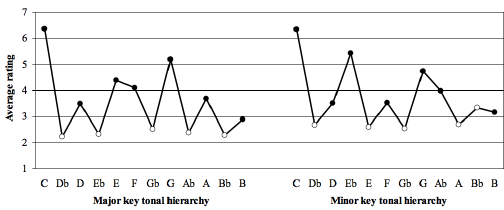
\includegraphics[width=.9\textwidth]{figs/key_profiles_C.png}
            \end{figure}
        \end{column}
    \end{columns}
\end{frame}

\subsection{Key Profiles}
\begin{frame}{Método}{Key Profiles}
    \begin{itemize}
        \item Krumhansl-Schmukler \& Kessler
        \begin{itemize}
            \item Análise subjetiva com voluntários 
            \item Quão bem uma nota soa num elemento musical de uma tonalidade (Escala, Cadência, etc)
            \item Contrução de um perfil tonal para todas as tonalidades maiores e outra para as menores
        \end{itemize}
        \item Temperley
        \item Bellman e Aarden
        \item Simple (Craig)
    \end{itemize}
\end{frame}

\subsection{Exemplo}
\begin{frame}{Método}{Exemplo}
    \begin{columns}[]
        \begin{column}{.5\textwidth}
            \begin{itemize}
                \item Melodia "Yankee Doodle"
                \item Construção da distruibuição
                \item Correlação com os perfis de Krumhansl
                \item Melhor previsão - G Major (0.693)
                \begin{itemize}
                    \item D Major (0.485)
                    \item E Minor (0.398)
                    \item G Minor (0.394)
                \end{itemize}
            \end{itemize}
        \end{column}
        \begin{column}{.5\textwidth}
            \begin{figure}
                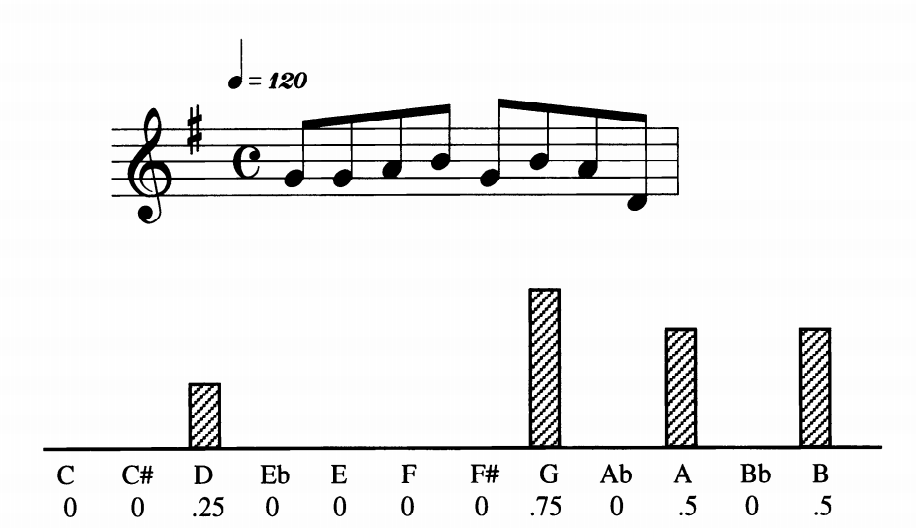
\includegraphics[width=.9\textwidth]{figs/yankee_song.png}
            \end{figure}
        \end{column}
    \end{columns}
\end{frame}
\section{Implementation} \label{sec:implementation}

Having described the algorithm, the next step is to implement it programmatically.
This is because if we want to obtain a significant number of results, doing calculations by hand would be impractical.

The implementation was done in Python, a high level programming language, with lots of libraries and tools for multimedia projects.
We made use of the library \textit{Music21}, a Python-based toolkit for computer-aided musicology \cite{music21}.

This library has a key determination algorithm implemented based on the \textit{Krumhansl-Schmuckler} key determination algorithm.
This is the one we will be making use in this project.

One advantage of this library is that it allows to specify which key-profiles to use when calculation the correlation with the sample.
This will allow us to compare different key profiles and their respective accuracy relatively easily.
For the purpose of the project, we will be explaining in relative detail how to use this library, detailing some classes and functions crucial in this project.

\subsection {music21.stream}

The class \textit{music21.stream} is the fundamental container in \textit{music21}.
It is in this class where objects may be ordered and/or placed in time based on offsets from the start of this container.
This means that it basically encodes music elements on a time-based system, effectively creating a file system that the rest of the library can understand.

Although it is possible to "manually" create a \textit{Stream}, defining which notes are to be played, as well as their time-frame, this is not necessary nor recommended.
What we will be doing in converting a music file into a \textit{Stream} using the function \textit{music21.converter.parse}.

This function accepts a number of symbolic music files, files where the data is structured, and therefore well defined if we know how to read it.
A few examples can be named like MusicXML, MuseData, Humdrum and most importantly, MIDI.

What is consistent amongst all these file types is that, although they store musical data, \textbf{none of them are in fact audio files}.
Although audio files, such as MP3 and WAV, enables us to play music in virtually any device, it does not contain any information regarding what is actually being played, 
i.e, we do not know whether a piano or a flute is playing simply by reading the file. This makes it very difficult to extract information like which notes are being played,
which is the essence of key determination for example.

For this matter, we use file types like MIDI, where all this information is available directly, simplifying significantly the process.
By parsing a MIDI file into a \textit{Stream}, we are know able to make use of the library's analyses function.
It is important to note that some equalization in applied in order to improve the algorithm's efficiency.
However, most excerpts will be unaffected as this equalization is done using a very high tempo subdivision.

\subsection{music21.analysis.discrete.KeyWeightKeyAnalysis} \label{sec:analysis_discrete}

Once we have created a \textbf{Stream} based on a MIDI file, we can now apply analysis tools to obtain different parameters.
One of such tools is the \textit{KeyWeightKeyAnalysis}, the implementation of the key determination algorithm.

To be precise, this class does not exist, i.e, you cannot define an object using this class. It is what is called a base class.
This means that for example classes \textit{...discrete.a} and \textit{...discrete.b}, both subclasses of \textit{...discrete.KeyWeightKeyAnalysis},
inherit the same base functions, although they can have specific functions for them.

The subclasses in this case will different key-profiles alternatives that can be applied in the algorithm:
\begin{itemize}
    \item SimpleWeights - Implementation of simple weights by Craig Sapp \cite{sapp2011computational}
    \item AardenEssen - Implementation of Aarden-Essen weightings \cite{aarden2003dynamic}
    \item BellmanBudge - Implementation of Bellman-Budge weightings \cite{bellmann2005determination}
    \item KrumhanslSchmuckler - Implementation of Krumhansl-Schmuckler/Kessler weightings \cite{krumhansl2001cognitive}
    \item TemperleyKostkaPayne - Implementation of Temperley-Kostka-Payne weightings \cite{Temperley2004Musicp}
\end{itemize}

Like mentioned before, this subclasses output a different correlation value as they make use of different key profiles.

Although not necessary, it is possible to see which profiles are being use for both major and minor keys in each implementation, by making use of the function \textit{KeyWeightKeyAnalysis.getWeights(weightType)}.
For example, this is the output of the Krumhansl-Schmuckler/Kessler weightings, represented in Figure \ref{fig:key_profiles_c}:

\begin{lstlisting}[language=bash]
    Major Key profile [6.35, 2.23, 3.48, 2.33, 4.38, 4.09, 2.52, 5.19, 2.39, 3.66, 2.29, 2.88]
    Minor Key profile [6.33, 2.68, 3.52, 5.38, 2.6, 3.53, 2.54, 4.75, 3.98, 2.69, 3.34, 3.17]
\end{lstlisting}

\subsection{music21.stream.analyze}

Although we can do the analysis by calling \ref{sec:analysis_discrete}, it is easier to simply call \textit{stream.analyze(arg)}.
This function runs a particular analytical method on the contents of the specified stream to find its key in this case, essentially calling \textit{music21.analysis.discrete.KeyWeightKeyAnalysis} functions.
For example, \textit{stream.analyze('key')} would output the prediction based on the implementation of Krumhansl-Schmuckler/Kessler weightings, which is the default one.
Making use of the subclass \textit{music21.analysis.discrete.analyzeStream}, we can specify which implementation we want to use.
This subclass matches the argument string with the implementations available:
\begin{itemize}
    \item analysis.discrete.analyzeStream(s, 'Krumhansl') = stream.analyze('Krumhansl') - Outputs prediction based on Krumhansl profiles
    \item analysis.discrete.analyzeStream(s, 'Temperley') = stream.analyze('Temperley') - Outputs prediction based on Temperley profiles
\end{itemize}

\subsection{music21.key.Key} \label{sec:key}

Independently of the method used to make the prediction the output will be an object of the class \textit{music21.key.Key}.
As described in the documentation, "Note that a key is a sort of hypothetical/conceptual object.
It probably has a scale (or scales) associated with it and a KeySignature, but not necessarily".

The \textbf{key signature} is the modification associated with a particular key in comparison to C Major. It is the number of sharps or flats it has.
For example, G Major's key signature has two sharps (F\# and C\#), while C Major has none.

A \textbf{scale} in the sequence of notes ordered by pitch starting from the key's tonic tonic and ending in the same (octave), taking into account the key signature of said key.
For example, G Major's scale is "G A B C\# D E F\# G", while C Major's is "C D E F G A B C".

These concepts are usually associated with tonal music, hence the small disclaimer in the documentation.
As only tonal music will be analysed, both parameters will be defined.

Although the above described functions will already output a \textbf{music21.key.Key} object, one can be easily defined:
\pagebreak

\begin{lstlisting}[language=bash]
    >> cm = key.Key('c')  # lowercase = c minor.
    >> cm
    <music21.key.Key of c minor>
    >>cm.mode
    'minor'
    >>cm.tonic.name
    'C'
    >>cm.sharps
    -2
    >>cm.pitches
    [<music21.pitch.Pitch C4>,
    <music21.pitch.Pitch D4>,
    <music21.pitch.Pitch E-4>,
    <music21.pitch.Pitch F4>,
    <music21.pitch.Pitch G4>,
    <music21.pitch.Pitch A-5>,
    <music21.pitch.Pitch B5>,
    <music21.pitch.Pitch C5>]
\end{lstlisting}

As observed, when we define a C Minor key, the object will have an associated key signature, as well as a scale.
All the returned objects form the analyses will be defined like this one, allowing us to make use of a large set of functions associated with this object.

The most important ones are arguably \textit{key.tonic.name} and \textit{key.mode}, which output the \textbf{pitch} (A, B, C, etc) and the \textbf{mode} (Major or Minor).
These are the two main parameters that will be used to analyse the precision of the algorithm. In short, \textbf{these define the key of the excerpt}.

Given that these parameters are output as \textit{strings}, a comparison can easily be made with the name of the file, which will contain the key itself (\textbf{Testing} section).

A number of other functions are also useful for this project.
\textit{key.relative} in a key object containing the relative of the main key. 
The \textbf{relative} in key that has the shares the same key signature as the main key, except the leading tone.
For example, the relative of G Major is E Minor, whose only difference is the D\#, the leading tone, which needs to be half-tone higher in minor keys.

Similarly, \textit{key.getDominant()} returns the \textbf{Dominant} pitch of the main key.
Although the Dominant does not share the same key signature, its tonic chord is a recurring presence in the main key, having therefore big similarities.
It is important to note that the object returned by this function is not \textit{music21.key.Key} but rather \textit{music21.pitch.Pitch}.
Although its brings different considerations into play, the dominant chord, and by extrapolation the key, is always major.
Therefore, we only need to know the pitch, which is similarly obtained using \textit{.name}.

Finally, \textit{key.parallel} returns a key object containing the \textbf{parallel} key of the main key. In short, its is the same pitch with opposite mode (A Major to A Minor).
The only thing these two keys share it a common tonic note, which can be enough to confuse the algorithm into prediction the parallel instead ot the main key.

The above described functions are the essential ones for this project, giving us all the information we need to make the necessary comparisons.
However, it is possible to go further into detail, in order to analyse the ambiguity of a prediction, for example.
In other words, how sure was the algorithm about its prediction: by a landslide, or was it a close match?
This information in related to the correlation value associated with each key.

This can be obtained using \textit{key.correlationCoefficient} for the chosen key.
If we want to know the results for the rest of the profiles, \textit{key.alternateInterpretations[n]} is a vector with the (n+2)-est best prediction.
Each of this entries is of course, a key object, so we can apply all the above functions on them as well:

\begin{lstlisting}[language=bash]
    Best Prediction =  A major 0.8769757225959743
    Second best Prediction =  G- minor 0.7810592206505336
    Third best Prediction =  E major 0.7077655748628783
    Worst Prediction =  E- major -0.7693194496397553
\end{lstlisting}

The above textbox shows the output for \textit{Prelude in A Major, J. S. Bach} using the Krumhansl key profile.
Not only do we see which one was the chosen key, but also the rest of podium, as well as the respective correlation values. 






\section{Evaluation} \label{sec:evaluation}

\subsection{Data set} \label{sec:data_set}
The first aspect to mention is the data set used.
In order to diversify the test, different sample groups were created and analysed separately.
This is because, if we are to make a fair judgement on the algorithms precision, we need to understand the theoretical implications each music sample has.

The first sample group is \textbf{J.S.Bach's Well Tempered Clavier}.
This is a compilation of 24 pieces written for each of the possible keys.
For this matter, it is an excellent data set as it goes through all possible solutions.

The second sample group in \textbf{F.Chopin's Études}.
Similarly, these 18 pieces have very diversified keys, presenting a good testing opportunity of the algorithm.
However, it is important to mention that Chopin and Bach have very different composition techniques.
This means that both data sets will bring different considerations.

The third sample group is \textbf{S.Rachmaninov's Piano Concertos 2 \& 3}.
Although this data set only has 6 samples (3 for each \textit{concerto}), they are much longer than previous ones.
This means that each sample is much more diverse and has more variations , making it much harder for the algorithm to predict the key.

The forth sample group is \textbf{Contemporary Music}, with 7 pieces including Debussy, Ravel and Satie.
This composers had a different understating of tonality, almost disregarding it.
In other words, given that the models were based on tonal perception, we expect that the algorithm will not do so well in this data set.

The last sample group is \textbf{Pop Music}, with 8 pieces.
This genre differs from the rest of the samples, as it is simpler and repetitive, even amongst themselves.
In fact, the chord progressing is most of the time very simple, consisting on perfect cadences that give away the key instantly.
Therefore, it is expected that the algorithm will do very well it this case.

\subsection{Analyses Considerations} \label{sec:analyses_considerations}
As mentioned before, although we will make use of the \citeauthor{krumhansl2001cognitive} algorithm, different key can be used.
We will test the precision of some of them, which are implemented in library we are using.

The different key profiles we will be testing are the ones mentioned in section \ref{sec:analysis_discrete}.

Not only will we evaluate the precision of the algorithm, i.e., if it predicted the right answer, but also analyse the wrong answers.
As mentioned in \ref{sec:key}, some key profiles are very similar to each other, namely:
\begin{itemize}
    \item Relative
    \item Dominant
    \item Parallel
\end{itemize}

Although still wrong answer, they are understandable mistakes because of the similarity, and analysing the excerpt might gives us some insights on the algorithm's output.

\subsection{Bach Analyses} \label{sec:bach}

\begin{center}
    \begin{tabular}{|c||c c c c c||} 
    \hline
    \% & Krum & Temp & Bell & Aard & Craig \\
    \hline\hline
    Correct & 100 & 100 & 100 & 100 & 100\\ 
    \hline
    Relative & 0 & 0 & 0 & 0 & 0\\
    \hline
    Dominant & 0 & 0 & 0 & 0 & 0\\
    \hline
    Parallel & 0 & 0 & 0 & 0 & 0\\
    \hline
    Other & 0 & 0 & 0 & 0 & 0\\
    \hline
   \end{tabular}
\end{center}

As we can observe from the table above, all the algorithms have 100\% accuracy. This is more-less to be expected.
The composition style in this pieces is very uniform. 
Perfect cadences are executed multiple times during the piece.
Perfect cadences correspond to the chord progression I - IV - V -I, which have all the major pitches in that key.
This way, because this pitches have a much higher weight in the analyses it will be easier to identify the key.

Another aspect to take consideration is modulations. Modulations consists in changing the main key of a section of the piece.
Bach often makes use of a modulation technique called \textit{Circle of fifths}.
This technique enables to modulation to many keys seamlessly to closely related keys.
These keys share many notes, and therefore do not impact much the prediction unless they are used very often.

Preludes should also be easier to analyse than Fugues, and in this case they were analysed together.

\subsection{Chopin Analyses} \label{sec:chopin}

\begin{center}
    \begin{tabular}{|c||c c c c c||} 
    \hline
    \% & Krum & Temp & Bell & Aard & Craig \\
    \hline\hline
    Correct & 94.44 & 94.44 & 94.44 & 94.44 & 100\\ 
    \hline
    Relative & 0 & 5.56 & 5.56 & 0 & 0\\
    \hline
    Dominant & 5.56 & 0 & 0 & 0 & 0\\
    \hline
    Parallel & 0 & 0 & 0 & 0 & 0\\
    \hline
    Other & 0 & 0 & 0 & 5.56 & 0\\
    \hline
   \end{tabular}
\end{center}

Although from a different age than Bach (Baroque), Chopin (Romantic) composed based on tonal rules and very fluently melodies and chords.
These meant that modulating were once again often used with closely related keys, like Dominant, sub-dominant and relative keys.
In these pieces in particular, modulating sections were long.

This explains while we see some predictions falling in other categories (the "other" prediction in "Aarden" was in fact to the sub-dominant).
It also needs to be taken into account that \textit{Études} are composed to train technique, often being simpler in terms of melody and harmonization.
These factors of course make it easier for the algorithm to work.


\subsection{Rachmaninov Analyses} \label{sec:rach}

\begin{center}
    \begin{tabular}{|c||c c c c c||} 
    \hline
    \% & Krum & Temp & Bell & Aard & Craig \\
    \hline\hline
    Correct & 16.67 & 33.33 & 33.33 & 33.33 & 33.33\\ 
    \hline
    Relative & 0 & 0 & 0 & 0 & 0\\
    \hline
    Dominant & 0 & 0 & 0 & 16.67 & 0\\
    \hline
    Parallel & 16.67 & 0 & 0 & 0 & 0\\
    \hline
    Other & 66.67 & 66.67 & 66.67 & 50 & 66.67\\
    \hline
   \end{tabular}
\end{center}

Rachmaninov piano concertos are the climax of the romantic period.
A period defined by emotions and a megalomaniacal Russian culture result in very intense and diverse music,
with these piano concertos being arguably the best representation of that.
Being such long pieces, we can identify different parts using different keys, techniques and tempos.
We can define these pieces as literally "All over the place" in terms on music composition.

Therefore, it is understandable the difficulty the algorithms have in correctly predicting the answer.
This category was in fact selected precisely to prove the major flaw in Krumhansl approach: no segmentation of the pieces.
When you have a long piece that modulates into different keys for long periods of time, it is impossible to predict the main key using this algorithm.
In fact it does not even make any sense to analyse these pieces in such a generic way, as their complexity calls for a more local approach.


\subsection{Contemporary Analyses} \label{sec:contemp}

\begin{center}
    \begin{tabular}{|c||c c c c c||} 
    \hline
    \% & Krum & Temp & Bell & Aard & Craig \\
    \hline\hline
    Correct & 57.14 & 57.14 & 57.14 & 42.86 & 57.14\\ 
    \hline
    Relative & 0 & 0 & 0 & 14.29 & 0\\
    \hline
    Dominant & 14.29 & 14.29 & 14.29 & 14.29 & 14.29\\
    \hline
    Parallel & 0 & 0 & 0 & 0 & 0\\
    \hline
    Other & 28.57 & 28.57 & 28.57 & 14.29 & 28.57\\
    \hline
   \end{tabular}
\end{center}

Contemporary music stands out for not following formal tonal music rules.
Although the pieces chosen are still from the early part of the movement, we can already identify, for example, that modulations do not make use of any technique in particular.
The composer bases its composition in the sonic effect rather than the formal modulation techniques.
For example, cadences are rarely perfect. In fact, tonal chords progressions are very rare.

As we are applying a tonal algorithm to "border-tonal" music, we can accept the 50\% accuracy obtained as a good performance from the algorithms. 
Especially considering that most mistakes were understandable, predicting the dominant of relative keys which, as explained in section \ref{sec:key}, have very similar profiles.
\subsection{Pop Analyses} \label{sec:pop}

\begin{center}
    \begin{tabular}{|c||c c c c c||} 
    \hline
    \% & Krum & Temp & Bell & Aard & Craig \\
    \hline\hline
    Correct & 75 & 75 & 100 & 100 & 87.5\\ 
    \hline
    Relative & 0 & 0 & 0 & 0 & 0\\
    \hline
    Dominant & 25 & 0 & 0 & 0 & 0\\
    \hline
    Parallel & 0 & 0 & 0 & 0 & 0\\
    \hline
    Other & 0 & 25 & 0 & 0 & 12.5\\
    \hline
   \end{tabular}
\end{center}

Pop music, as mentioned before, is very simple and makes use of repetitive chord progressions.
Modulations are rarely made, and when they are, it is using closely related keys.
Because these keys all share most pitches in common, some mistakes are understandable.
However some algorithms got 100\% accuracy, proving that in fact, this is the easiest genre to analyse.
Bach might seem to be better, but Bach's sample list was bigger than Pop's.
Therefore a direct comparison is not possible.
As argument can be made given the fact that analysing by hand a piece of Bach might take a day, while Pop music takes 1 minute.



\subsection{Profile Comparison} \label{sec:total_analyses}

\begin{center}
    \begin{tabular}{|c||c c c c c||} 
    \hline
    \% & Krum & Temp & Bell & Aard & Craig \\
    \hline\hline
    Correct & 68.65 & 71.98 & 76.98 & 74.13 & 75.59\\ 
    \hline
    Relative & 0 & 1.11 & 1.11 & 2.86 & 0\\
    \hline
    Dominant & 8.96 & 2.86 & 2.86 & 6.19 & 2.86\\
    \hline
    Parallel & 3.33 & 0 & 0 & 0 & 0\\
    \hline
    Other & 19.06 & 24.05 & 19.05 & 16.82 & 21.55\\
    \hline
   \end{tabular}
\end{center}

Comparing the average performance of the different algorithms, the original algorithm, Krumhansl, has the worst performance,
while Bellman's key profiles have the best results by a significant margin.

The original key profiles were based completely in a subjective analyses done with volunteers based on "sounding nice".
Although this might work most of the time, it only goes so far, as complex musical properties come into play when the excerpts are more complex.
It is expected that, with more technology and more research, newer models were suggested after studying the original model and identifying its flaws.

Another aspect to take into consideration is the type of weights given to each key.
In Krumhansl, the tonic has a weight of 6.35, with the next pitch (not part of the scale of that key) having a weight of 2.23.
In Aarden, the tonic weights 17.7661, with next pitch weighting 0.145624.

We can see that in Aarden / Bellman profiles, much bigger importance is given to the notes that are part of the scale of that pitch, in contrast with Krumhansl / Temperley.
This reduces the error caused by ornamentations of passing notes.
Simple (Craig) profiles give 0 weight to pitches that are not part of the scale and 1 to the ones that are, with the tonic weighting 2.

Given that the sample list is not that extended and/or diverse, the algorithms can be said to be performing at more less the same level,
with the revisions slightly outperforming in some more complex categories.
\section{Conclusão}
\begin{frame}{Conclusão}{}
    \begin{itemize}
        \item Fundamentos teóricos da Tonalidade
        \item Algoritmos de deteção
        \begin{itemize}
            \item Krumhansl-Schmukler
        \end{itemize}
        \item Key Profiles
        \begin{itemize}
            \item Krumhansl
            \item Temperley
            \item etc.
        \end{itemize}
        \item Implementação em Python
        \begin{itemize}
            \item Music21
        \end{itemize}
        \item Análise de precisão
        \begin{itemize}
            \item Melhorias no algoritmo
        \end{itemize}
    \end{itemize}
\end{frame}







% \section*{Acknowledgments}
%The authors would like to thank...




\printbibliography[]

\end{document}
